\documentclass[]{article}

% Imported Packages
%------------------------------------------------------------------------------
\usepackage{amssymb}
\usepackage{amstext}
\usepackage{amsthm}
\usepackage{amsmath}
\usepackage{enumerate}
\usepackage{fancyhdr}
\usepackage{float}
\usepackage[margin=1in]{geometry}
\usepackage{graphicx}
\usepackage{extarrows}
\usepackage{setspace}
%------------------------------------------------------------------------------

% Header and Footer
%------------------------------------------------------------------------------
\pagestyle{plain}
\renewcommand\headrulewidth{0.4pt}
\renewcommand\footrulewidth{0.4pt}
%------------------------------------------------------------------------------

% Title Details
%------------------------------------------------------------------------------
\title{
  Erudite\\
  \large \emph{An educational content management system}\\
  \vspace{1em}
  High-Level Architectural Design
}
\author{
  SE 3A04: Software Design II -- Large System Design
  \\
  \begin{tabular}{ l l }
    Kelvin Lin*   & STUDENT-NUM \\
    Danish Khan   & STUDENT-NUM \\
    Puru Jetly    & STUDENT-NUM \\
    Terrance Yip  & STUDENT-NUM \\
    Varun Hooda   & STUDENT-NUM \\
  \end{tabular}
}
\date{}
%------------------------------------------------------------------------------

% Document
%------------------------------------------------------------------------------
\begin{document}

\maketitle
\newpage

\tableofcontents
\newpage

\section{Introduction}
\label{sec:introduction}
This section outlines the purpose and provides a system description of the
Erudite project; along with an overview of the contents and organization of
this detailed design document.


\subsection{Purpose}
\label{sub:purpose}
The purpose of this document is to give outline the detailed design of the
Erudite system; including a description of the system's behaviour, interactions
of the subsystems and components, and finally a detailed outline of all the
classes that will compose this system as a whole.

The target audience for this document are the stakeholders (Dr. Ridha Khedri,
Andrew LeClair and Michael Liut), and any current or future architects,
designers and developers of this project.


\subsection{System Description}
\label{sub:system_description}
The Erudite application is intended to be an educational content management
system for use in elementary school classrooms. The primary interface between
the user and the software system is through a device running the Android
operating system. This document defines the way in which the users will be
expected to interact with the system and how the application will be decomposed
into smaller subsystems to reduce the complexity and improve the
maintainability, flexibility of this system.

Specifically, the users of this system (application) are expected to perform a
set of events that will prompt the system to react. The decomposition will then
show how the subsystems will communicate among one another in order to
efficiently distribute the work and perform the required actions in response to
the user's actions.


\subsection{Overview}
\label{sub:overview}
The remainder of this document is organized into 3 sections: State Charts for
Controller Classes -- defining the behaviour of the controller classes,
Sequence Diagrams -- outlining the sequence of interactions between different
subsystems for various \underline{\bf scenarios/business events??}, and
Detailed Class Diagram -- specifying the classes that will compose the system,
the relations between classes and the methods each class provides. Each section
uses appropriate UML diagrams to describe and document the design details.

% End Section

\section{State Charts for Controller Classes}
\label{sec:state_charts_for_controller_classes}
% Begin Section
The following section contains state charts for each controller class in Erudite.

\subsection{The Main Controller}
{
\begin{figure}[H]
  \centering
  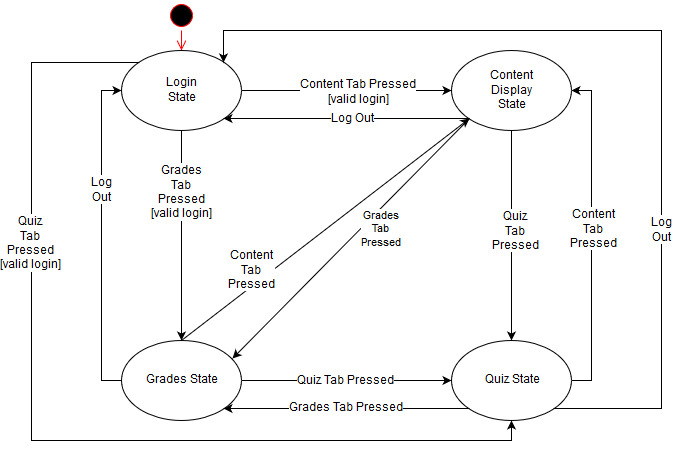
\includegraphics[scale=0.5]{A3_Assets/MainController.jpg}
  \caption{Main Controller State Chart}
\end{figure}
}

\subsection{The Login Controller}
{
\begin{figure}[H]
  \centering
  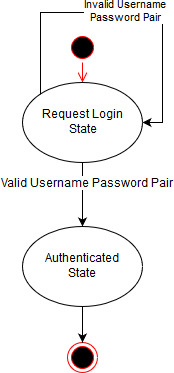
\includegraphics[scale=0.5]{A3_Assets/LoginController.jpg}
  \caption{Login Controller State Chart}
\end{figure}
}

\subsection{The Content Controller}
{
\begin{figure}[H]
  \centering
  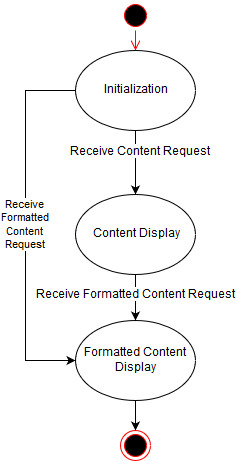
\includegraphics[scale=0.5]{A3_Assets/ContentController.jpg}
  \caption{Content Controller State Chart}
\end{figure}
}

\subsection{The Quiz Controller}
{
\begin{figure}[H]
  \centering
  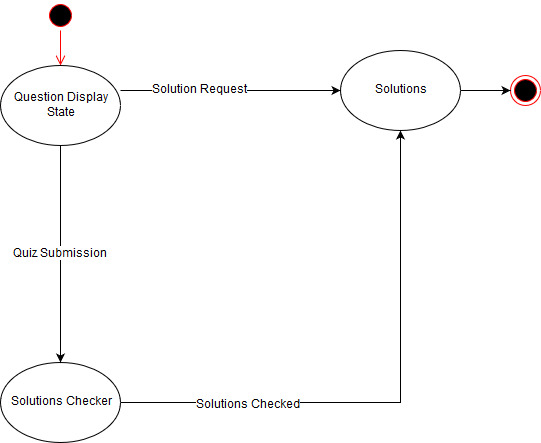
\includegraphics[scale=0.5]{A3_Assets/QuizController.jpg}
  \caption{Quiz Controller State Chart}
\end{figure}
}

\subsection{The Grades Controller}
{
\begin{figure}[H]
  \centering
  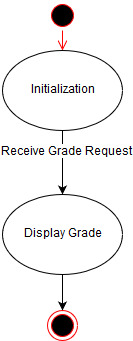
\includegraphics[scale=0.5]{A3_Assets/GradeController.jpg}
  \caption{Grades Controller State Chart}
\end{figure}
}
% End Section

\section{Sequence Diagrams}
\label{sec:sequence_diagrams}
% Begin Section
This section contains sequence diagrams for each use case identified in Deliverables 1 and 2.

\subsection{Student Logs In}
{
\begin{figure}[H]
  \centering
  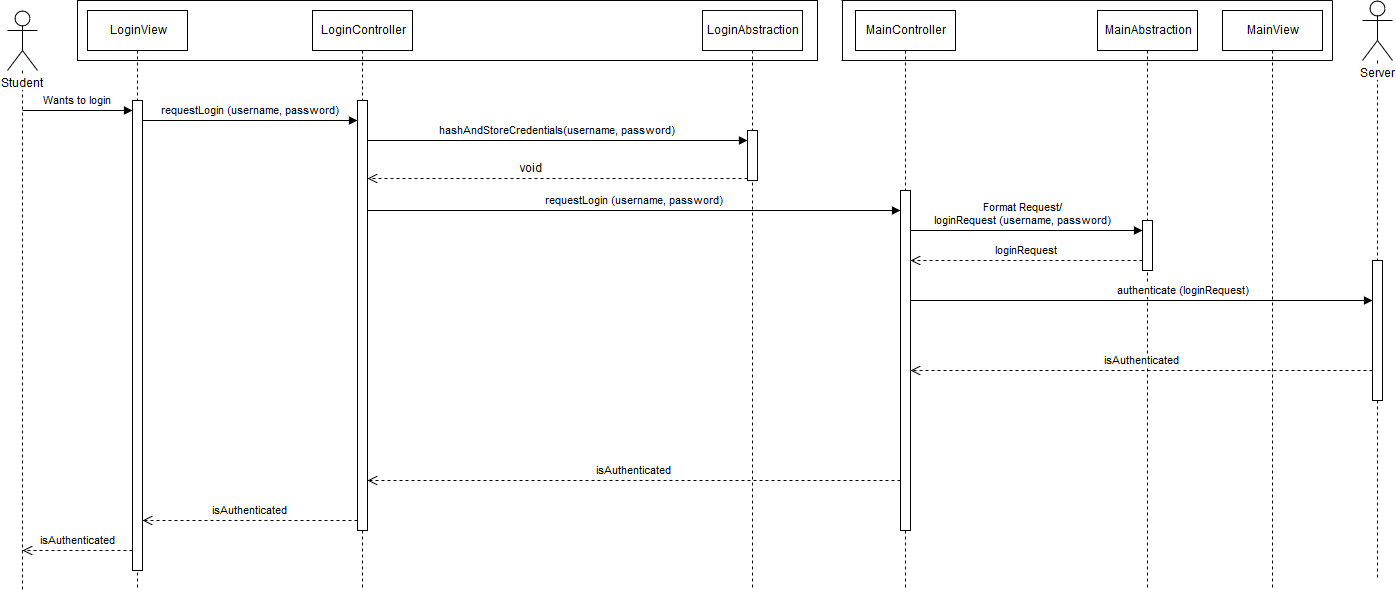
\includegraphics[scale=0.3]{A3_Assets/StudentLogsIn.jpg}
  \caption{Student Logs In Sequence Diagram}
\end{figure}
}

\subsection{Student Opens Content}
{
\begin{figure}[H]
  \centering
  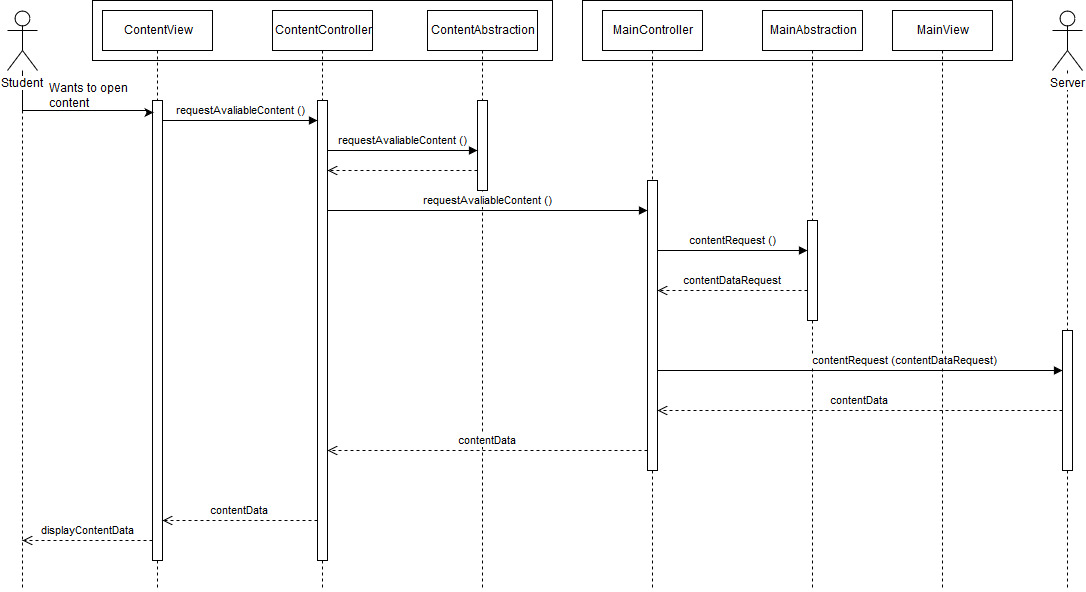
\includegraphics[scale=0.3]{A3_Assets/StudentOpensContent.jpg}
  \caption{Student Opens Content Sequence Diagram}
\end{figure}
}

\subsection{Student Submits Assignment}
{
\begin{figure}[H]
  \centering
  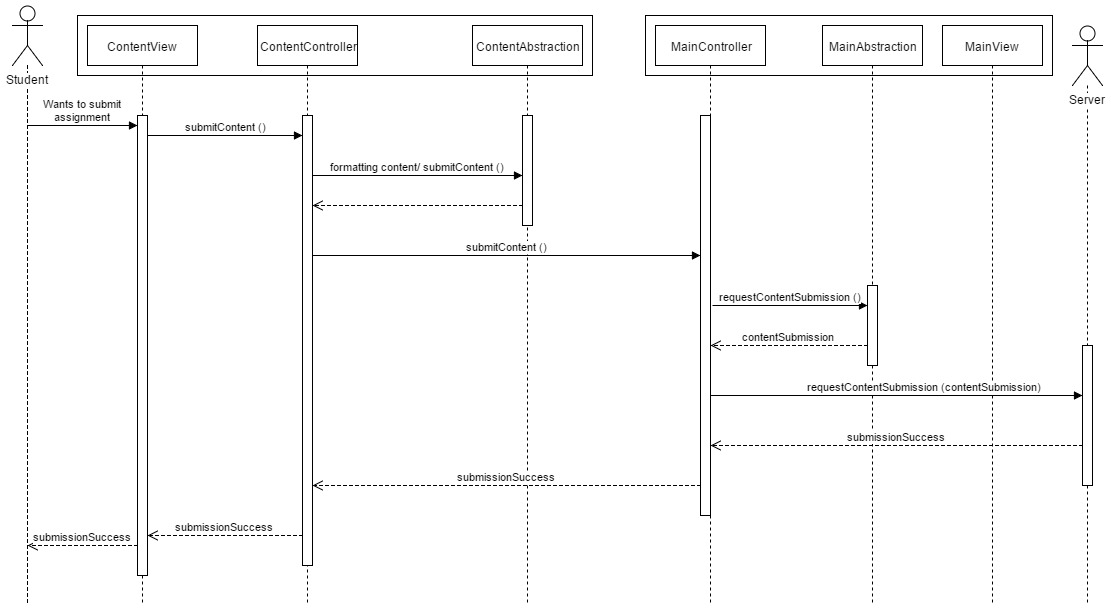
\includegraphics[scale=0.3]{A3_Assets/StudentSubmitsAssignment.jpg}
  \caption{Student Submits Assignment Sequence Diagram}
\end{figure}
}

\subsection{Student Opens Quiz}
{
\begin{figure}[H]
  \centering
  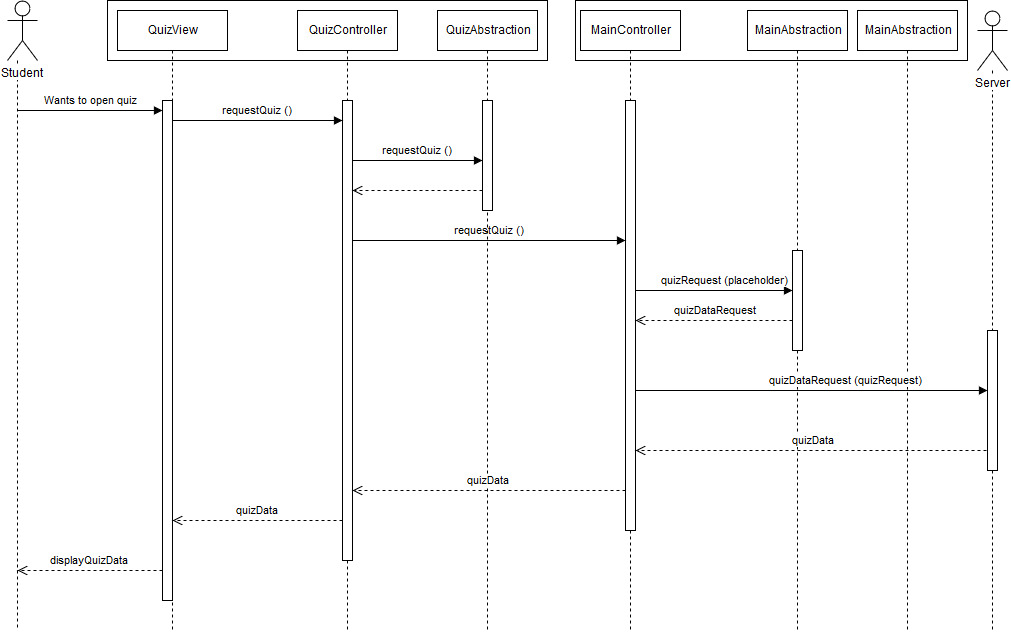
\includegraphics[scale=0.3]{A3_Assets/StudentOpensQuiz.jpg}
  \caption{Student Opens Quiz Sequence Diagram}
\end{figure}
}

\subsection{Student Completes Quiz}
{
\begin{figure}[H]
  \centering
  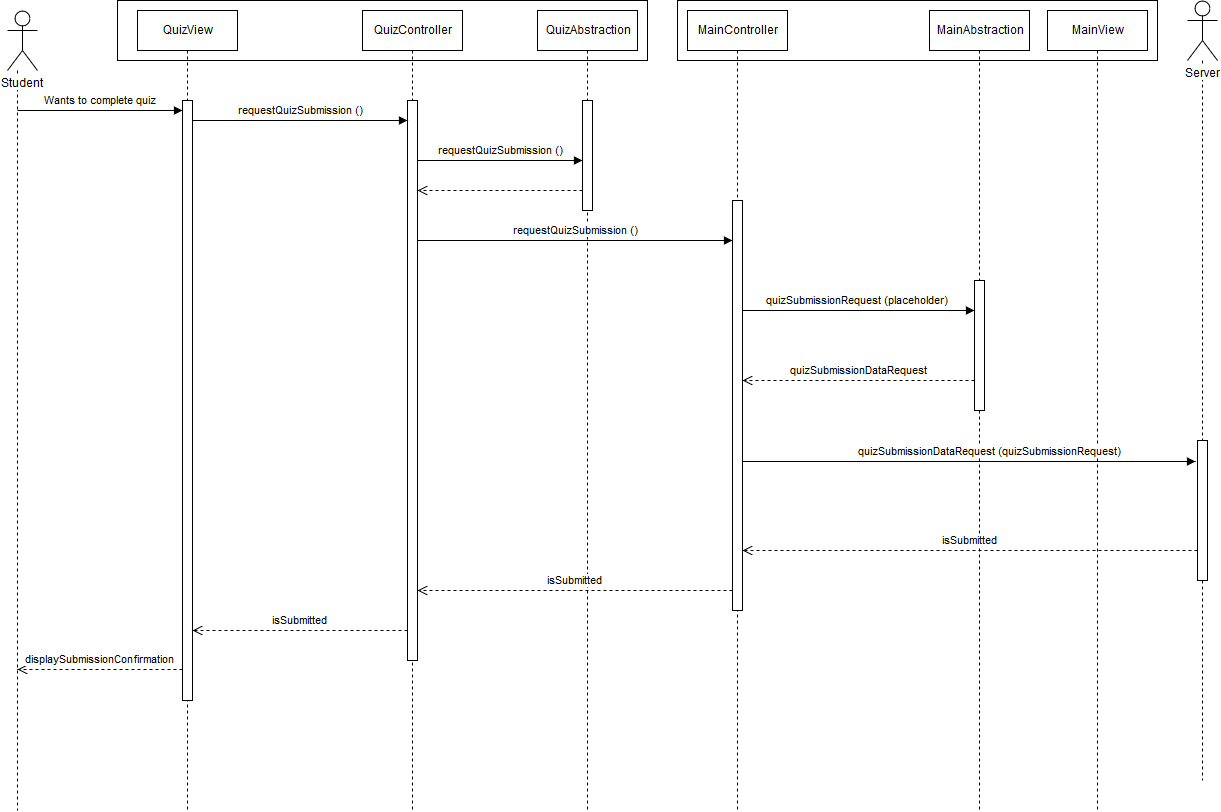
\includegraphics[scale=0.3]{A3_Assets/StudentCompletesQuiz.jpg}
  \caption{Student Completes Quiz Sequence Diagram}
\end{figure}
}

\subsection{Student Checks Grade}
{
\begin{figure}[H]
  \centering
  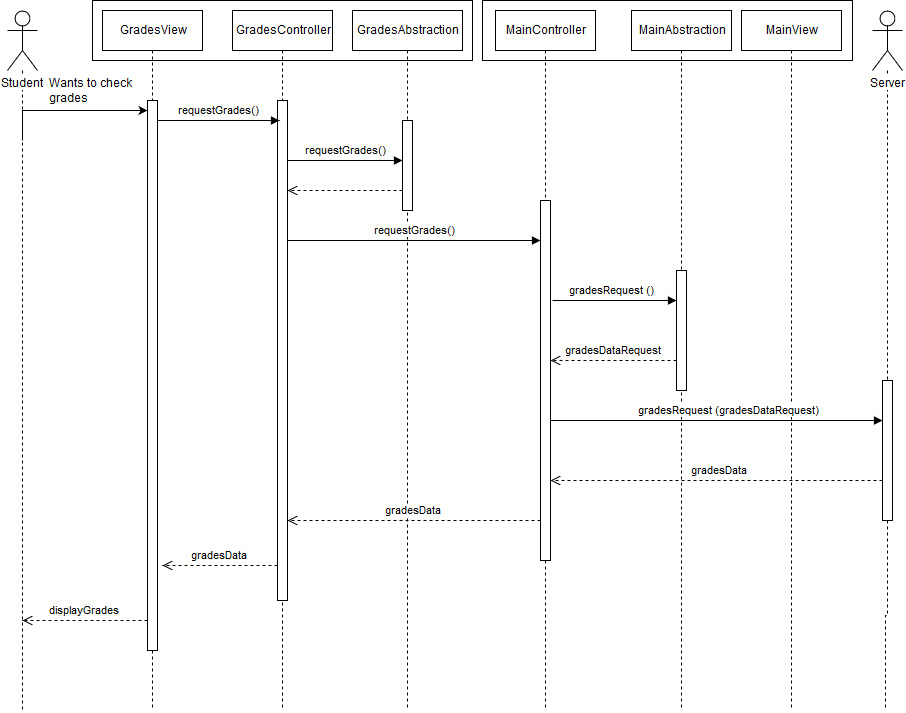
\includegraphics[scale=0.3]{A3_Assets/StudentChecksGrades.jpg}
  \caption{Student Checks Grade Sequence Diagram}
\end{figure}
}

\subsection{Teacher Logs In}
{
\begin{figure}[H]
  \centering
  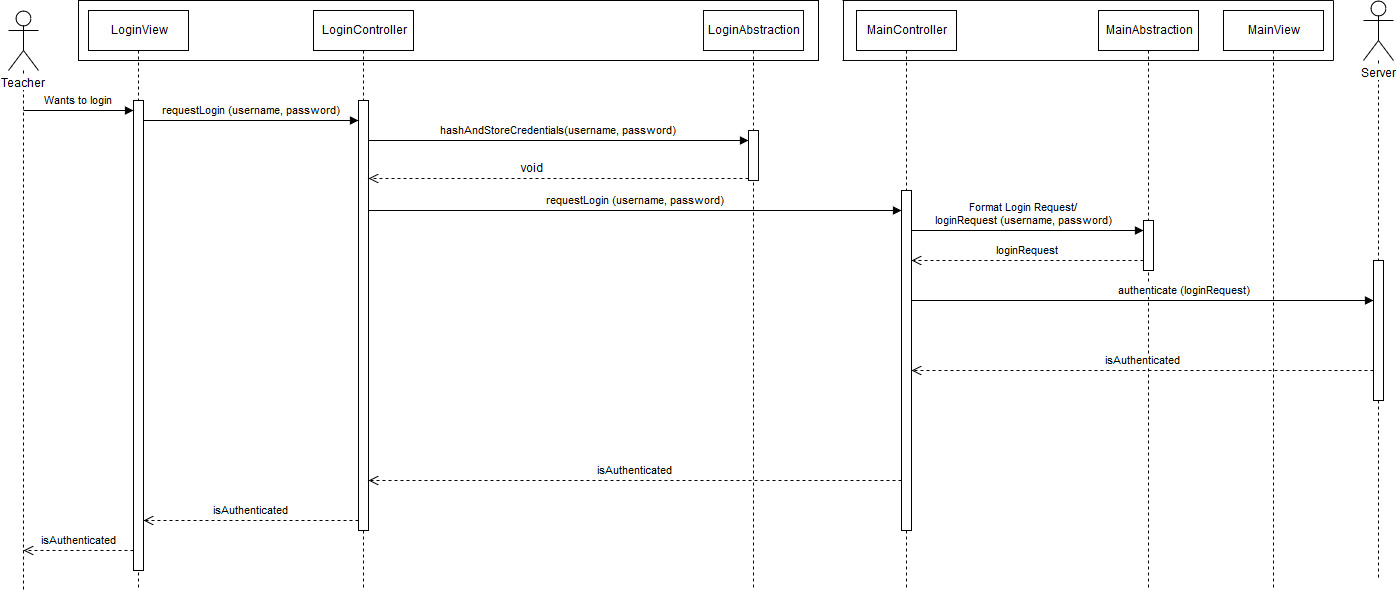
\includegraphics[scale=0.3]{A3_Assets/TeacherLogsIn.jpg}
  \caption{Teacher Logs In Sequence Diagram}
\end{figure}
}

\subsection{Teacher Opens Content}
{
\begin{figure}[H]
  \centering
  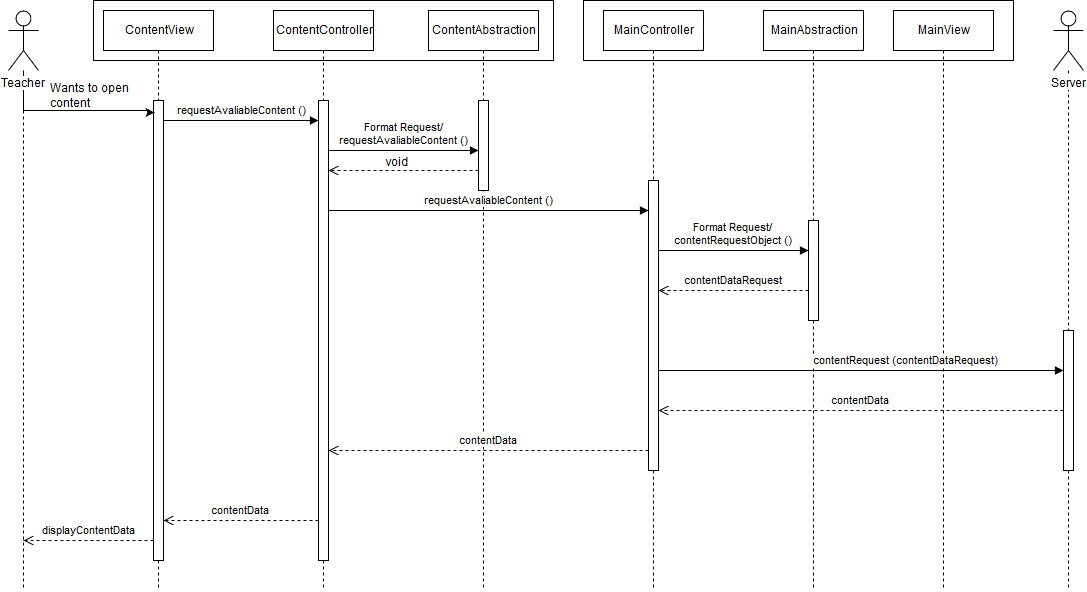
\includegraphics[scale=0.3]{A3_Assets/TeacherOpensContent.jpg}
  \caption{Teacher Opens Content Sequence Diagram}
\end{figure}
}
% End Section

\section{Detailed Class Diagram}
\label{sec:detailed_class_diagram}
% Begin Section
The following is a detailed class diagram for Erudite.
\begin{figure}[H]
  \centering
  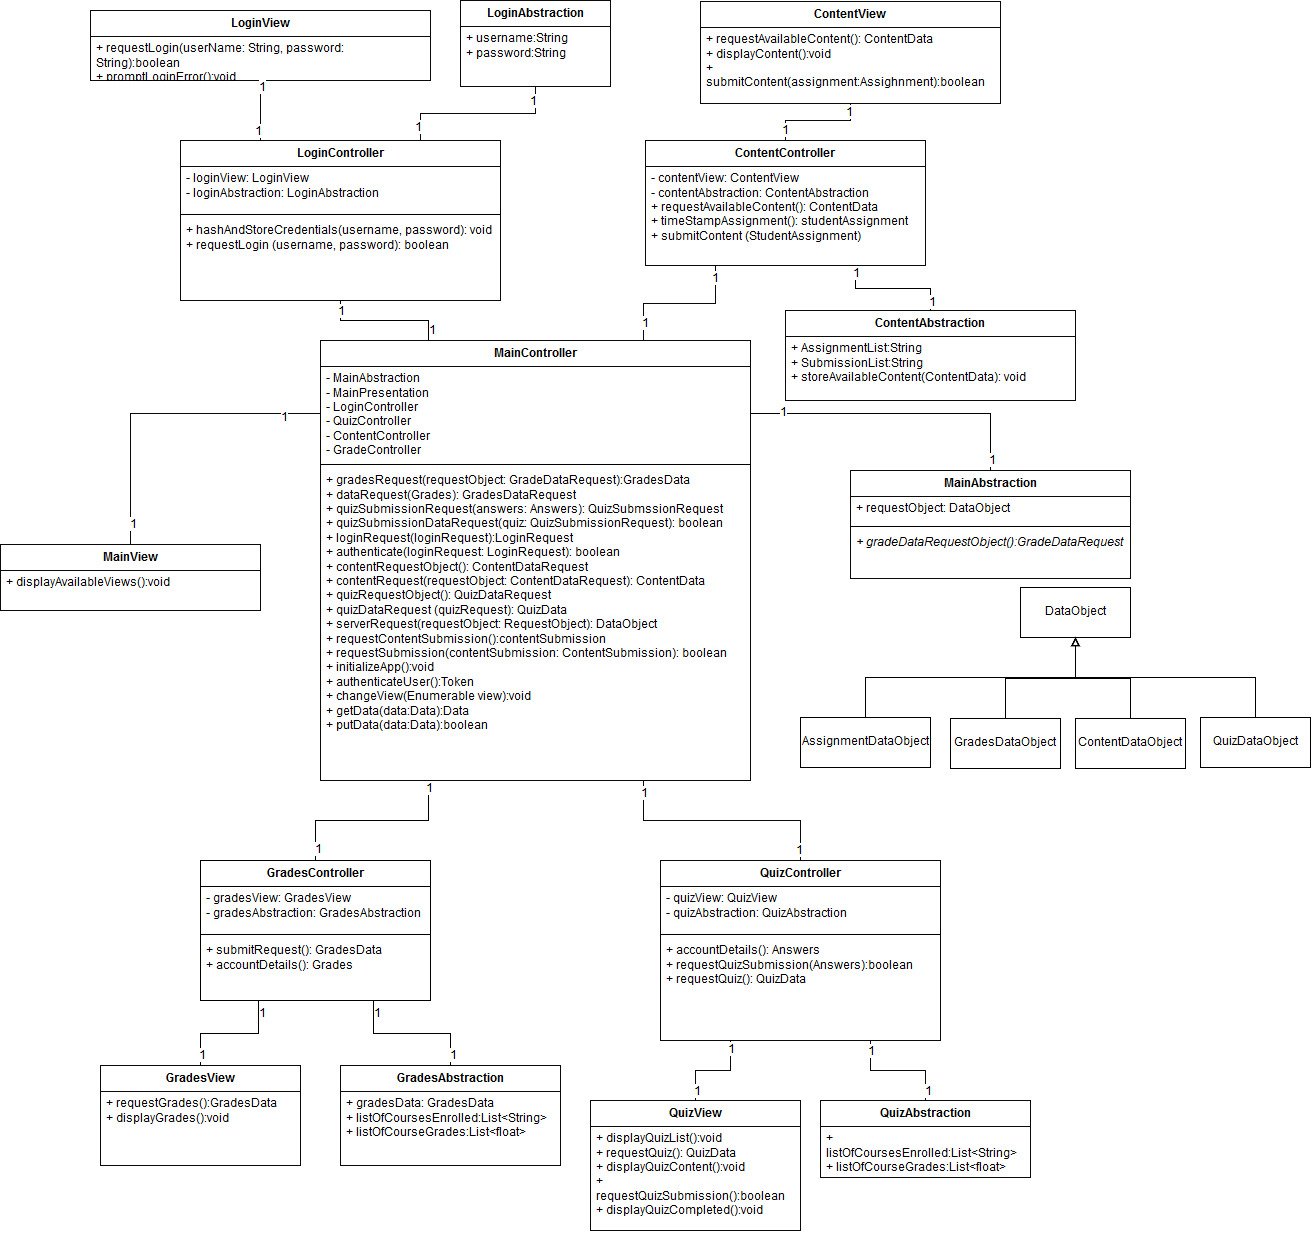
\includegraphics[scale=0.3]{A3_Assets/DetailedClassDiagram.jpg}
  \caption{Detailed Class Diagram}
\end{figure}
% End Section


\newpage
\appendix
\section{Division of Labour}
\label{sec:division_of_labour}
\begin{description}
  \item [Kelvin Lin ]
  \item Created State Chart Diagrams
  \item Consolidated all diagrams to final document
  \item Updated Deliverable 2 CRC Cards
  \hfill \rule{2in}{0.1pt}
  \\\\

  \item [Danish Khan]
  \item Detailed Class Diagram
  \item Collaborated on Sequence Class Diagram
  \hfill \rule{2in}{0.1pt}
  \\\\

  \item [Puru Jetly]
  \item foo
  \hfill \rule{2in}{0.1pt}
  \\\\

  \item [Terrance Yip]
  \item foo
  \hfill \rule{2in}{0.1pt}
  \\\\

  \item [Varun Hooda]
  \item{Section 1 Introduction}
  \item{Collaborated on Detailed Class Diagram}
  \hfill \rule{2in}{0.1pt}
  \\\\
\end{description}


% \newpage
% \section*{IMPORTANT NOTES}
% \begin{itemize}
%   \item You do \underline{NOT} need to provide a text explanation of each diagram; the diagram should speak for itself
%   \item Please document any non-standard notations that you may have used
%   \begin{itemize}
%     \item \emph{Rule of Thumb}: if you feel there is any doubt surrounding the meaning of your notations, document them
%   \end{itemize}
%   \item Some diagrams may be difficult to fit into one page
%   \begin{itemize}
%     \item It is OK if the text is small but please ensure that it is readable when printed
%     \item If you need to break a diagram onto multiple pages, please adopt a system of doing so and throughly explain how it can be reconnected from one page to the next; if you are unsure about this, please ask me
%   \end{itemize}
%   \item Please submit the latest version of Deliverable 1 and Deliverable 2 with Deliverable 3
%   \begin{itemize}
%     \item They do not have to be a freshly printed versions; the latest marked versions are OK
%   \end{itemize}
%   \item If you do \underline{NOT} have a Division of Labour sheet, your deliverable will \underline{NOT} be marked
% \end{itemize}


\end{document}
%------------------------------------------------------------------------------
